\subsection{coalesced thread access}
In this exersise we copy data from device to device using a for loop and multiple threads accessing memory in a coalesced manner.
First we utilize only one threadblock and vary the number of threads. Using more threads, we expectedly increase the rate
at which we are able to copy data from global to global memory. The amount of parallelism increases with more threads.
The advantage is small at small data sizes but increases ever larger at larger datasizes as we have less overhead.
We reach peak transfer speeds with 1024 threads already quite early at 1MB with around 18 GB/s with 1024 threads,
after which the performance drops. Possibly this could have something to do with the size of the L2 cache of around
1MB, where with data larger than 1MB the threads have to deal with slower and multiple accesses to main memory.

\begin{figure}
    \centering
    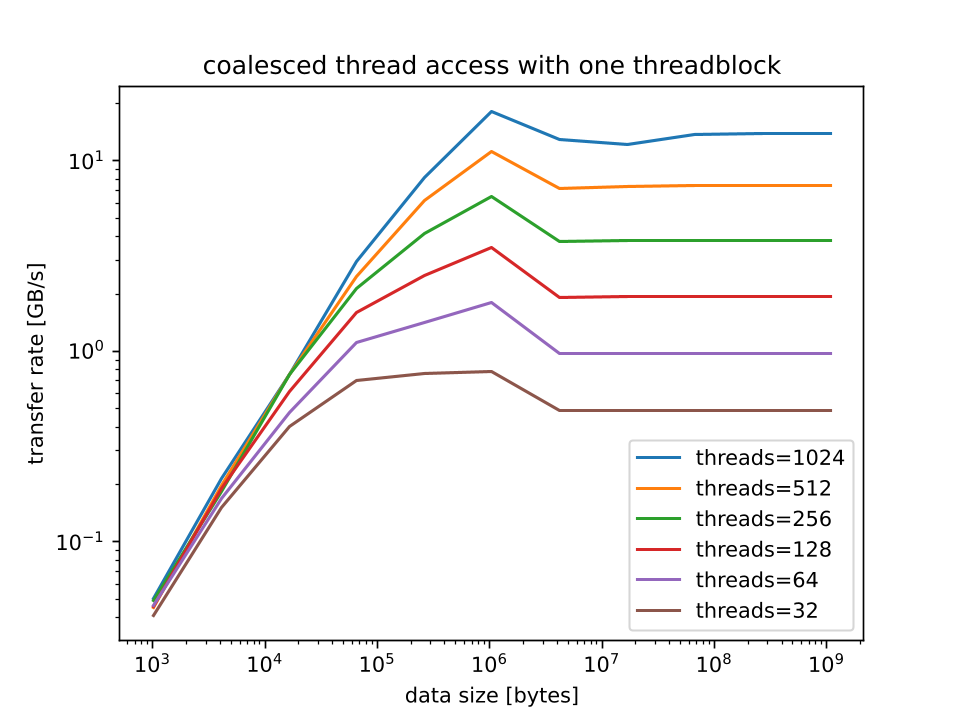
\includegraphics[scale=0.7]{pictures/coalesced_thread_access_a.png}
    \caption{exercise 2.2: 1 threadblock, different numbers of threads}
    \label{fig:2.2a}
\end{figure}

Next we varied the number of threadblocks for the peak-performing 1024 threads. Also here we can see the advantage
of more threadblocks emerge only at larger data sizes. Peak performance is reached with the maximum 32 threadblocks at
a data size of 67MB with 212 GB/s, close to the cudaMemcpy bandwidth. More parallelism in this case also means higher transfer speeds.
As with varying the number of threads, the performance is best at a few MB but drops slightly when reaching even larger data sizes around 1GB.
Again this could have to do with the size of the L2 cache. The optimal performance was reached with the maximum number of threads (1024) and
threadblocks (32).

\begin{figure}
    \centering
    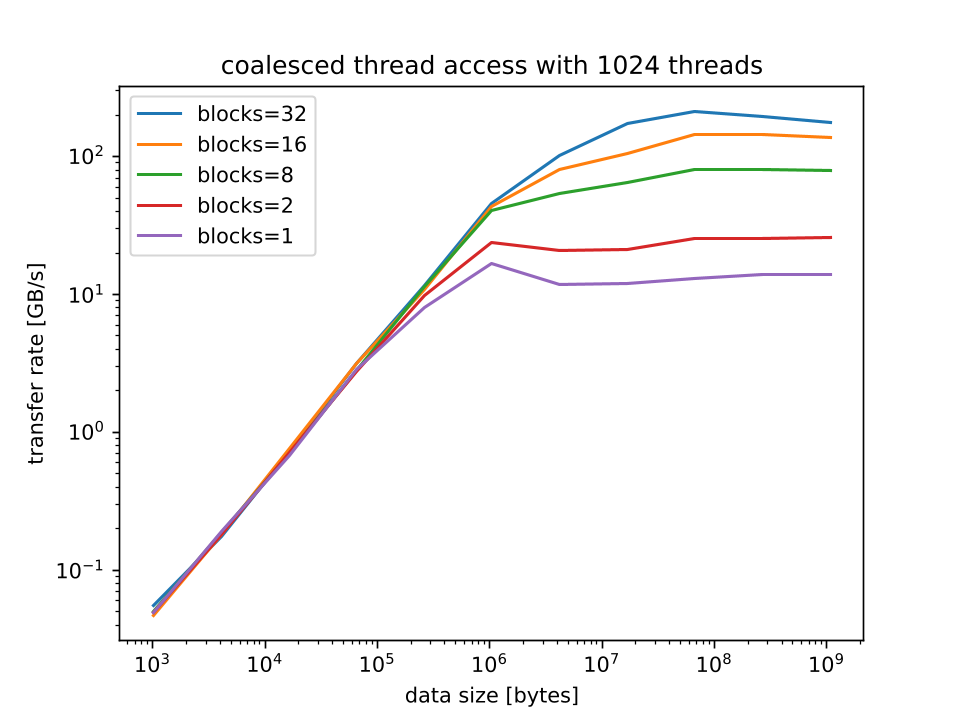
\includegraphics[scale=0.7]{pictures/coalesced_thread_access_b.png}
    \caption{exercise 2.2: 1024 threads, different numbers of blocks}
    \label{fig:2.2b}
\end{figure}